\hsection{Cloning git Repositories with the git Client}%
%
\begin{figure}%
\centering%
%
\subfloat[][%
After opening the \ubuntu\ \linux\ \pgls{terminal} using \ubuntuTerminal, we enter the directory into which we want to download the repository. %
We then type the command \bashil{git clone https://github.com/thomasWeise/databasesCode} and hit \keys{\return}. %
The option \bashil{--recurse-submodules} can be added just in case.%
\label{fig:gitCloneClient1clone}%
]{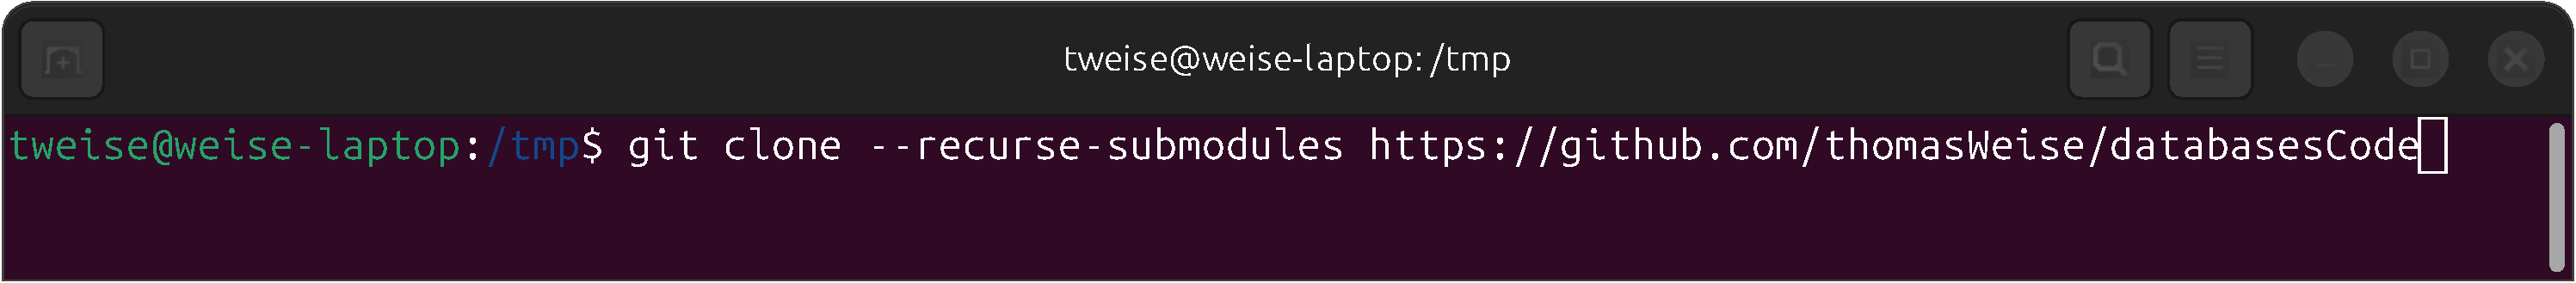
\includegraphics[width=0.78\linewidth]{\currentDir/gitCloneClient1clone}}%
%
\floatRowSep%
%
\subfloat[][%
The process of cloning the repository begins.%
\label{fig:gitCloneClient2cloning}%
]{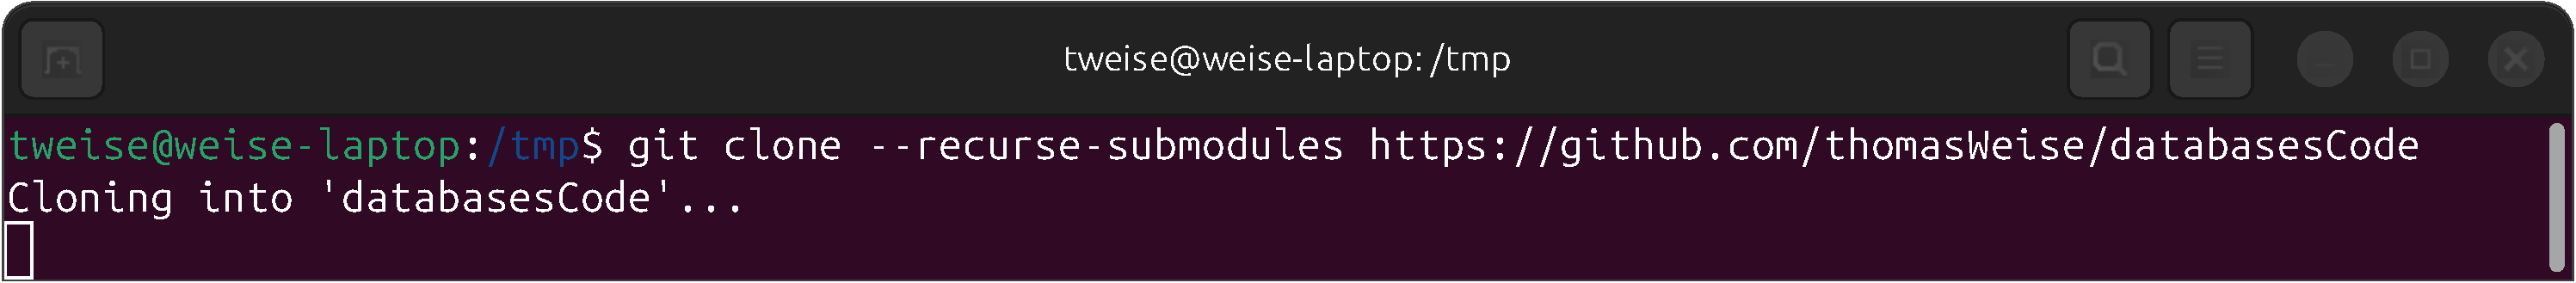
\includegraphics[width=0.78\linewidth]{\currentDir/gitCloneClient2cloning}}%
%
\floatRowSep%
%
\subfloat[][%
Sometimes, there may be connectivity issues. %
But do not fret if that happens\dots%
\label{fig:gitCloneClient3error}%
]{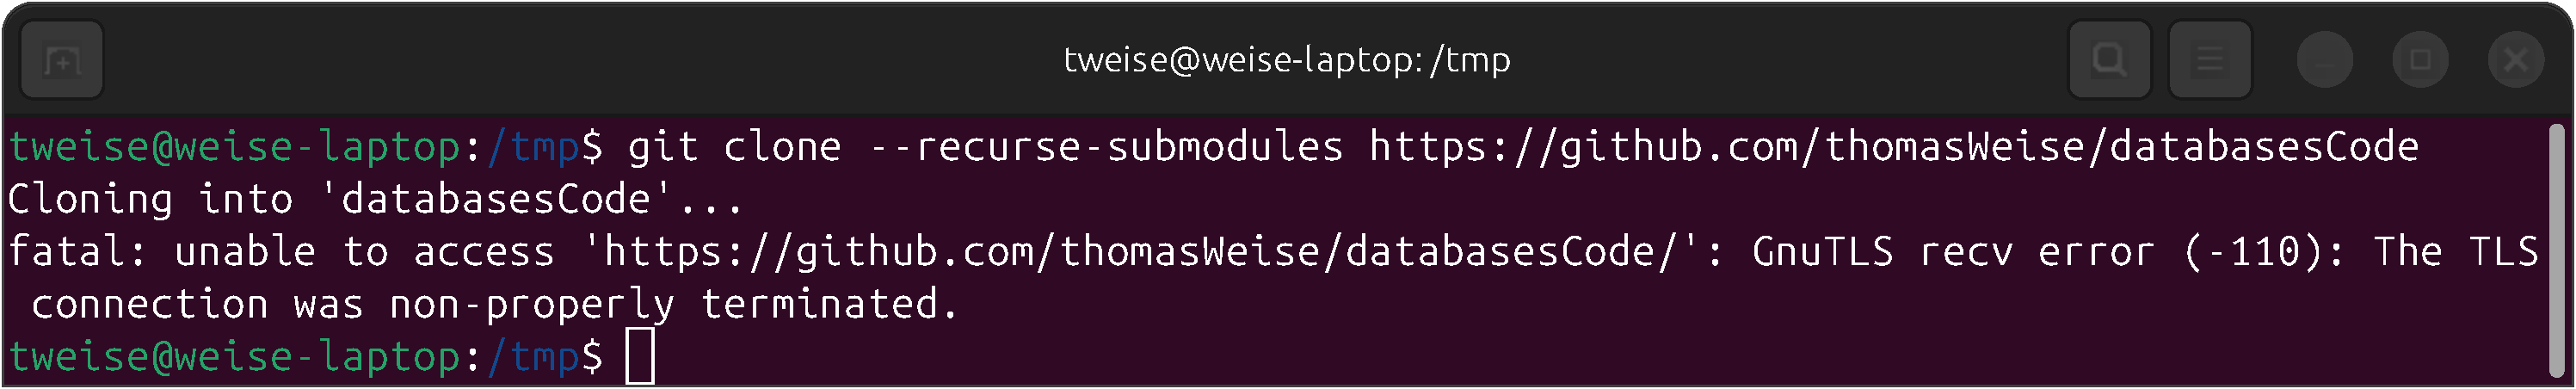
\includegraphics[width=0.78\linewidth]{\currentDir/gitCloneClient3error}}%
%
\floatRowSep%
%
\subfloat[][%
{\dots}simply try again (and, if necessary, again and again). %
Sometimes, it may make sense to switch the network, e.g., from using WLAN, instead connect your mobile phone to your computer using a USB cable and share the data connection of the mobile phone using USB tethering.%
\label{fig:gitCloneClient4nextAttempt}%
]{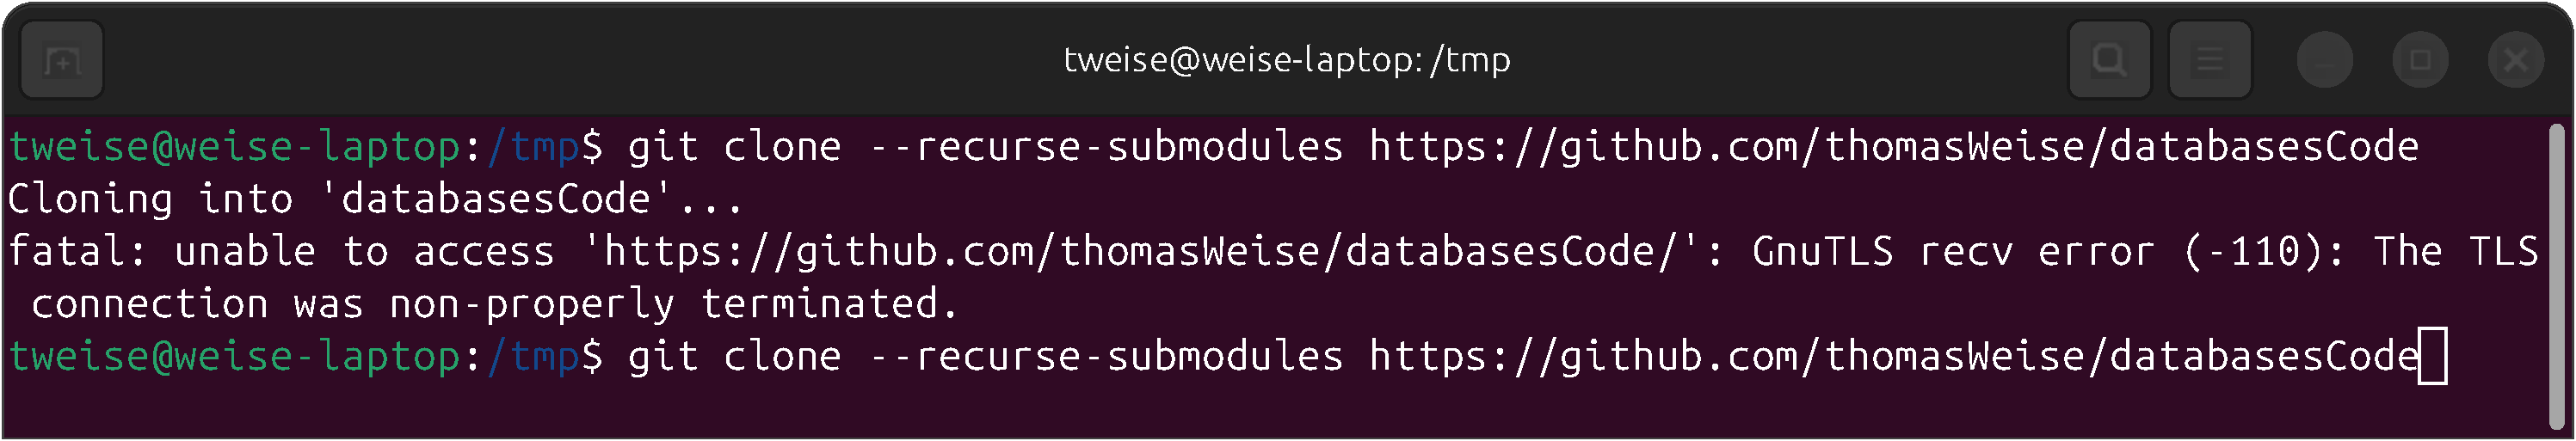
\includegraphics[width=0.78\linewidth]{\currentDir/gitCloneClient4nextAttempt}}%
%
\floatRowSep%
%
\subfloat[][%
Eventually, it will work.%
\label{fig:gitCloneClient5success}%
]{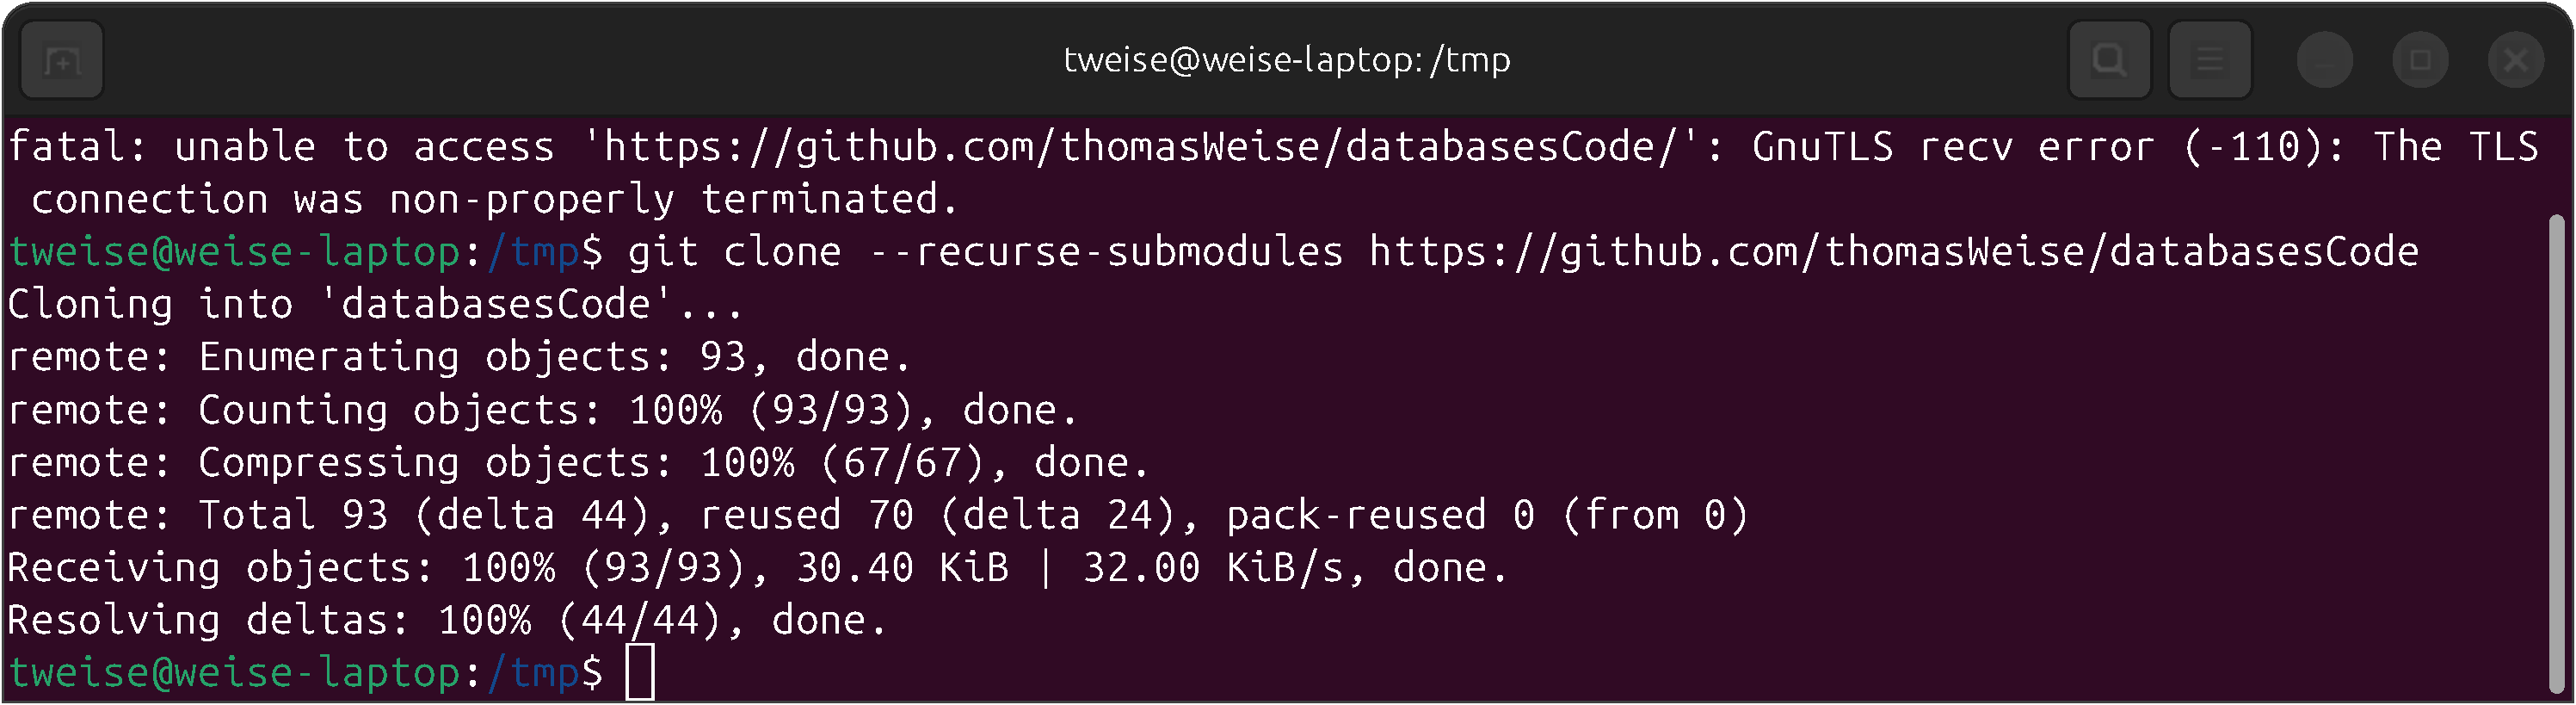
\includegraphics[width=0.78\linewidth]{\currentDir/gitCloneClient5success}}%
%
\floatRowSep%
%
\subfloat[][%
The repository has been downloaded and a new folder with the repository name (here:~\textil{databasesCode}) has appeared.%
\label{fig:gitCloneClient6files}%
]{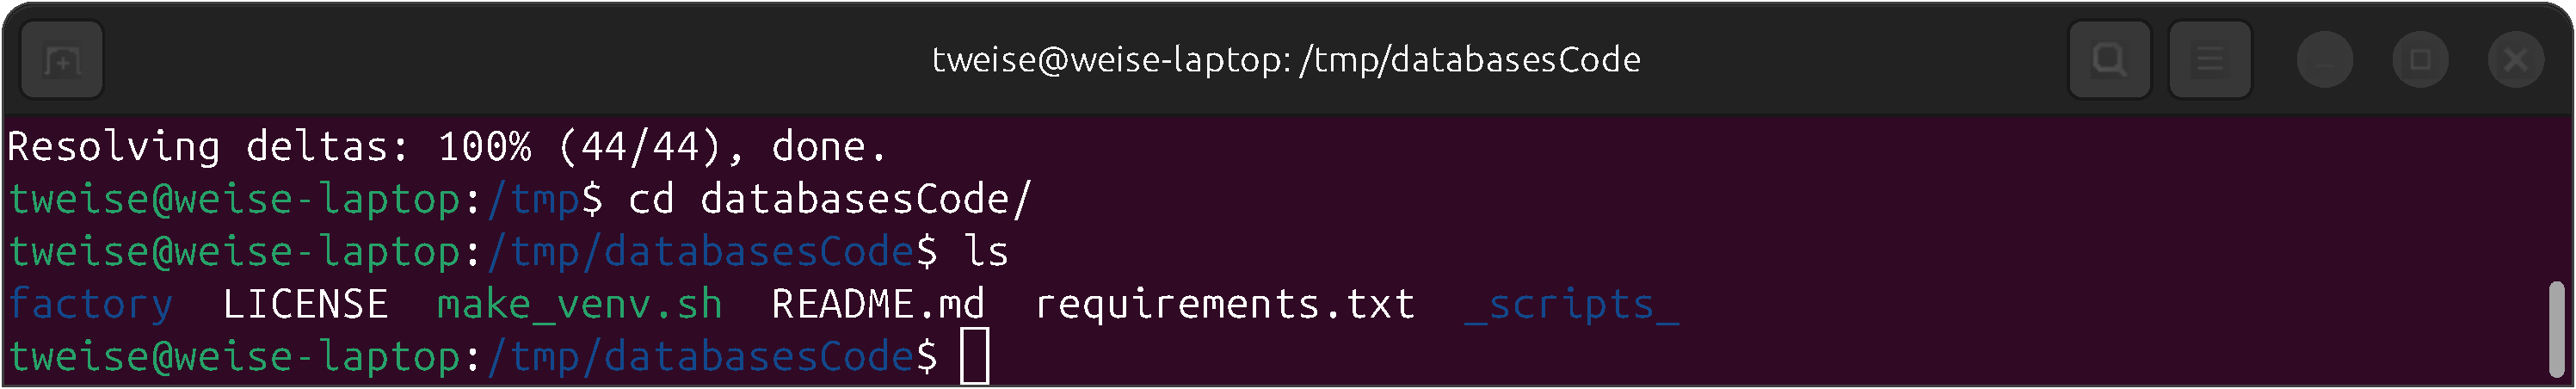
\includegraphics[width=0.78\linewidth]{\currentDir/gitCloneClient6files}}%
%
\caption{Cloning a \git\ repository using the \git\ \pgls{client} application \bashil{git} in an \ubuntu\ \linux\ \pgls{terminal} and how to deal with connection errors.}%
\label{fig:gitCloneClient}%
%
\end{figure}%
%
The most basic way to clone \git\ repositories is to use the \git\ \pgls{client} application.
This is a command line tool that can be executed in a \pgls{terminal}.
Here, we simply assume that you already have it installed the \git\ \pgls{client} program~\bashil{git}.

In \cref{fig:gitCloneClient}, we illustrate how the \git\ \pgls{client} program is used under \ubuntu\ \linux.
Under \microsoftWindows, it will work analogously.
First, we need to open a \pgls{terminal} window.
Under \ubuntu\ \linux, we therefore press \ubuntuTerminal.
Under \microsoftWindows, we instead \windowsTerminal.
We then enter the directory into which we want to download the repository using~\bashil{cd}.
Notice that if we download a repository with the name~\textil{abc}, this will create a new directory named~\textil{abc} inside that current working directory.

We then type the command \bashil{git clone https://github.com/thomasWeise/databasesCode} and hit \keys{\return}.
Sometimes, repositories contain submodules.
A submodules is basically a links to a specific state (commit) of \emph{another} repository.
The files of the referenced commit of the other repository would then exist inside a directory of the repository that we want to clone.
If we want to have a full copy of all the files, including the files referenced this way, we need to add the option \bashil{--recurse-submodules} to the \bashil{git} command.
We do this in \cref{fig:gitCloneClient1clone} to be on the safe side for demonstration purpose (although the repository \textil{databasesCode} does \emph{not} have any submodule).

After we hit \keys{\return}, the process of cloning the repository begins in \cref{fig:gitCloneClient2cloning}.
Sadly, when we clone repositories using \pgls{HTTPS} \pglspl{URL} from \github, sometimes, there may be connectivity issues.
I noticed that using the \pgls{SSH} \pglspl{URL} is much more reliable.
An example for such an error is shown in \cref{fig:gitCloneClient3error}.

However, this is not a big problem.
If such errors happen, you can simply try again after some time.
I furthermore noticed that, often, changing your internet connection can solve the problem.
Let's say that you are trying to clone the repository using your wired or wireless LAN and it does not work.
Then it often helps to first switch of the network connection on your computer.
On your mobile phone, you should also switch off wireless LAN and instead activate your mobile data connection.
Then you can connect your mobile phone to your computer using a USB cable and select \emph{USB tethering} on your phone.
This will share the mobile data connection with your computer.
Then, simply try to clone the repository again, as shown in \cref{fig:gitCloneClient4nextAttempt}.
The connection switching is just a quick work around.
Often, \bashil{git clone} works at first attempt and, if not, works after you wait a minute or so.

Eventually, it will work, as shown in \cref{fig:gitCloneClient5success}.
After the \bashil{git} command completes, the repository has been downloaded and a new folder with the repository name (here:~\textil{databasesCode}) has appeared.
The \bash\ command \bashil{ls} lists the files in a directory.
We see that the new directory contains the downloaded files in \cref{fig:gitCloneClient6files}.
Here, we will not deal with the issue of \pglspl{virtualEnvironment}, as we discussed them in the previous section about cloning repositories using \pycharm.%
%
\FloatBarrier%
\endhsection%
